\documentclass[t,english]{sdqbeamer}
%\documentclass[c]{sdqbeamer}

\usepackage{listings}
\usepackage{graphicx}
\usepackage{tabularx}
\usepackage{tikzsymbols}
\usepackage{booktabs}
\usepackage{forloop}

\usepackage[lined,linesnumbered,ruled,noend]{algorithm2e}
\renewcommand{\thealgocf}{}

\hypersetup{
	colorlinks=true,
	urlcolor=kit-green,
	citecolor=mygray
}

% set sdqbeamer options
\titleimage{blender-render}
\groupname{} % rendered at the bottom center of each slide
\grouplogo{ae+satres}
\selectlanguage{english}

% define title etc.pp.
\title{Practical SAT Solving}
\subtitle{Lecture 10 \unimp{\normalfont -- Planning \& Model Checking}}
\author{{Ashlin Iser}, \underline{Dominik Schreiber}}
\date{July 7, 2025}

% define commands
\input{l00-commands.tex}

%\usepackage[english]{babel}
\usepackage[citestyle=numeric,bibstyle=numeric,hyperref,backend=biber,language=auto]{biblatex}
\addbibresource{references.bib}
\bibhang1em
\setbeamertemplate{navigation symbols}{}

\setlength{\itemsep}{1em}
%\setbeamertemplate{itemize subitem}{\normalsize\insertsubitem}

\newcommand{\iflecture}[1]{#1}
\newcommand{\ifresearchtalk}[1]{#1}

\begin{document}

\begin{frame}[title white horizontal, picture=logos/blender-render, kitlogo=rgb]
	\titlepage
\end{frame}

\begin{frame}{Overview}
	\begin{block}{Recap Lecture 9}
		\begin{itemize}
			\item Common state-of-the-art \highl{proof formats}
			\item Pragmatics of \highl{proof production} and \highl{checking}
			\item Producing proofs with \highl{parallel + distributed solvers}
			\item Beyond proof files: \highl{on-the-fly checking}
		\end{itemize}
	\end{block}
	\begin{blueblock}{Today: Applications I}
		\begin{itemize}
			\item Why consider applications?
			\item Automated planning: Foundations and SAT-based methods
			\item From planning to checking: Bounded Model Checking basics
		\end{itemize}
	\end{blueblock}
\end{frame}






\begin{frame}{Why consider the Application View? (1/2)}
	
	\vspace*{-2mm}
	\centering
	%\small
	\begin{tabular}{llll}
		\toprule
		\multicolumn{2}{l}{\textbf{Result, instance family}} & \textbf{1st author} & \textbf{Speedups of \textsc{MallobSat} over \textsc{Kissat-MAB\_HyWalk}} \\
		\midrule
		% "Kakuro"; very large, sharing long clauses
		SAT & Hypertree decomposition 					 & Schidler & 3, 5, 5, 5, 5, 7, 8, 9, 12, 13 \\
		% lowest speedups are where the seq. solver is reasonably fast (100s)
		SAT & Hamilton circle 							 & Heule & 4, 4, 7, 11, 17, 20, 21, 22, 24, 31, 33, 36, 42 \\
		% very large, sharing long clauses
		SAT & Tree decomposition 						 & Ehlers & 5, 7, 87 \\
		% sharing pretty long clauses; pretty large inputs which the seq. solver solves reasonably quickly
		UNSAT & Cellular automatons 						 & Chowdhury & 5, 8, 8, 9, 9, 10, 22, 22, 66 \\
		\multicolumn{4}{c}{\vdots} \\[1mm]
		% Only clauses of length <= 4 shared
		UNSAT & Relativized pidgeon hole				 & Elffers & 277, 542, 638 \\
		UNSAT & Bioinformatics 							 & Bonet & 292, 717 \\
		UNSAT & Balanced random 					 & Spence & 321, 388 \\
		% ONLY sharing unit clauses for two highest speedups!
		SAT & Sum of three cubes 					 & Riveros & 384, 509, 1018, 3345 \\
		\unimp{SAT} & \unimp{Circuit multiplication} & \unimp{Shunyang} & \unimp{17, 31, 32, 62, 105, 119, 213, 254, 393, 741, 746, 1401, 2650} \\
		% heavy use of cardinality constraints - Probably Lingeling. Highest speedups: solved in <1s
		\unimp{UNSAT} & \unimp{Perfect matchings} 		 & \unimp{Reeves} & \unimp{119, 413, 12\,439, 108\,593, 217\,099} \\
		\bottomrule
	\end{tabular}
	
	\vspace*{3mm}
	\unimp{\small
		3072 cores (128 machines) of SuperMUC-NG\ \ $\cdot$\ \ 400 problems from Int. SAT Competition 2021\\
		Only instances with seq.\ time $\geq 60\,$s\ \ $\cdot$\ \ Only families with $\geq 2$ instances
	}
\end{frame}

\begin{frame}{Why consider the Application View? (2/2)}
	\vspace*{-4mm}
	\begin{itemize}
		\item Perform \highl{sound \textbf{algorithm engineering}} with \highlo{realistic applications} in the loop
		\item Understand \highl{application-specific solver behavior}, needs, shortcomings
		\item Advance the \highl{positive feedback loop between solvers and applications}
	\end{itemize}
	
	\vspace*{6mm}
	%\centering
	\hspace*{2cm}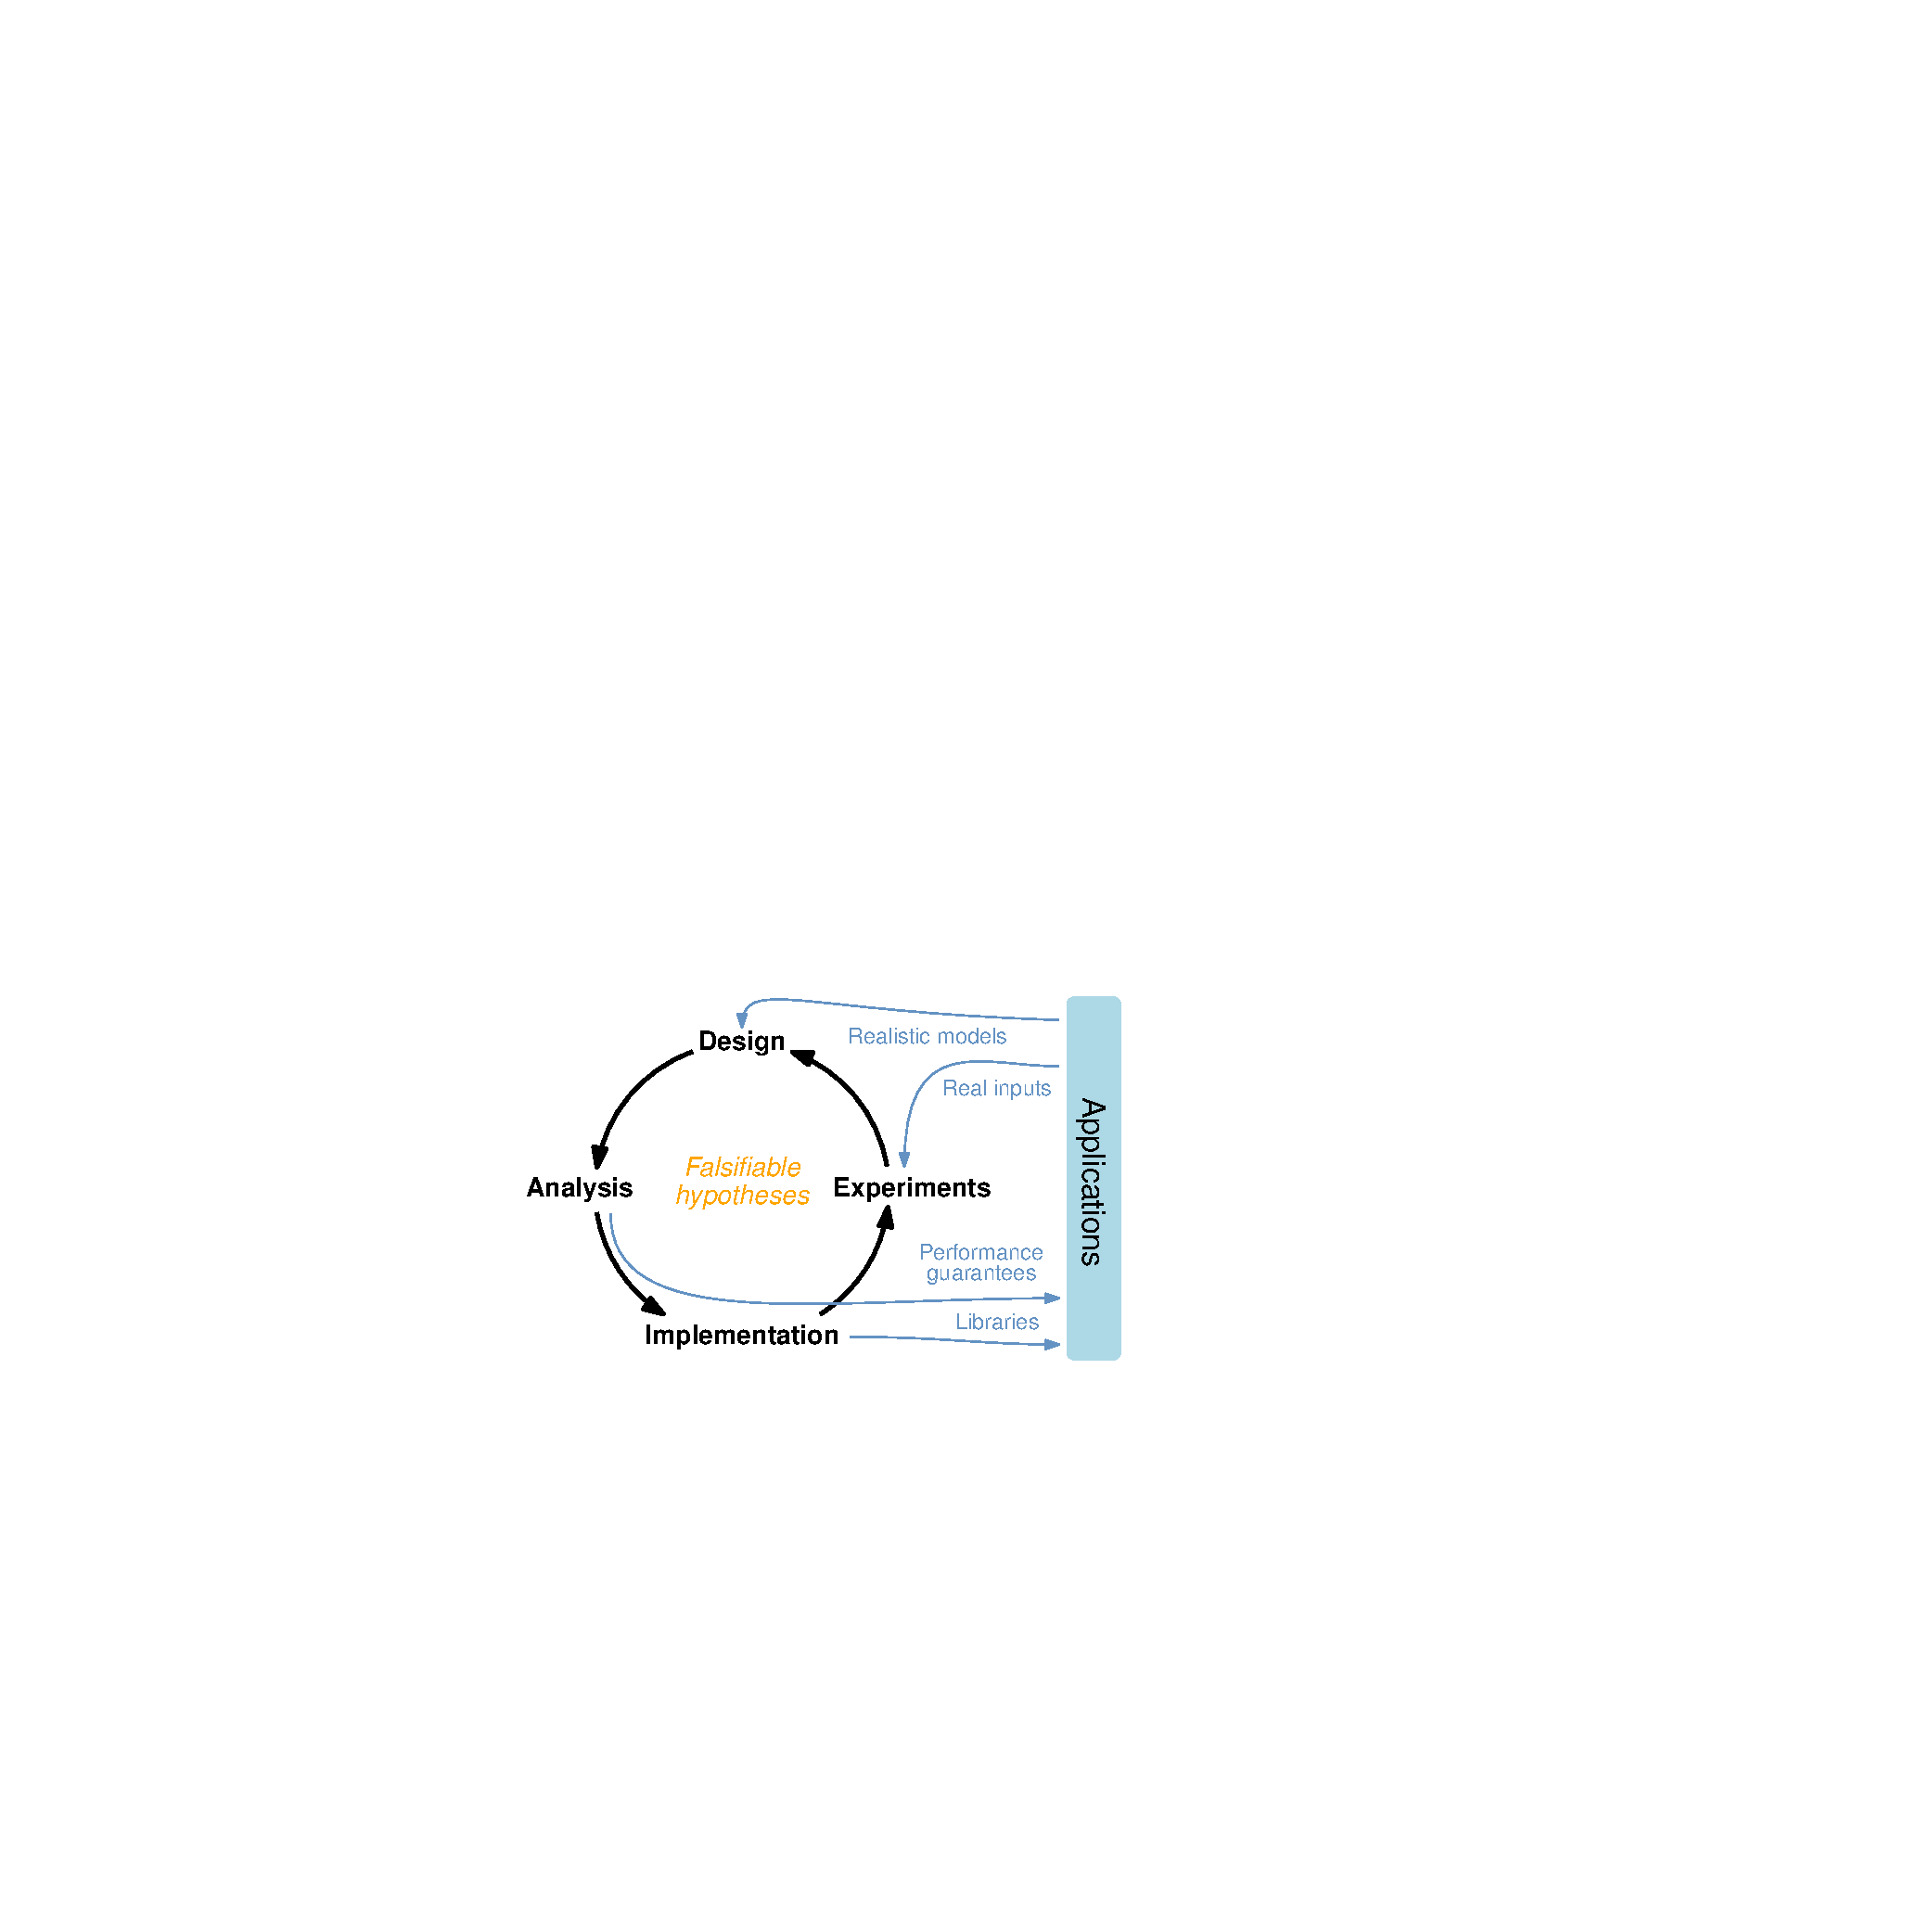
\includegraphics[width=0.5\textwidth]{figures/l10/algorithm-engineering.pdf}
\end{frame}

\begin{frame}{SAT Competition Benchmarks -- ``Real'' Applications?}
	\begin{minipage}{0.73\textwidth}
		\centering
		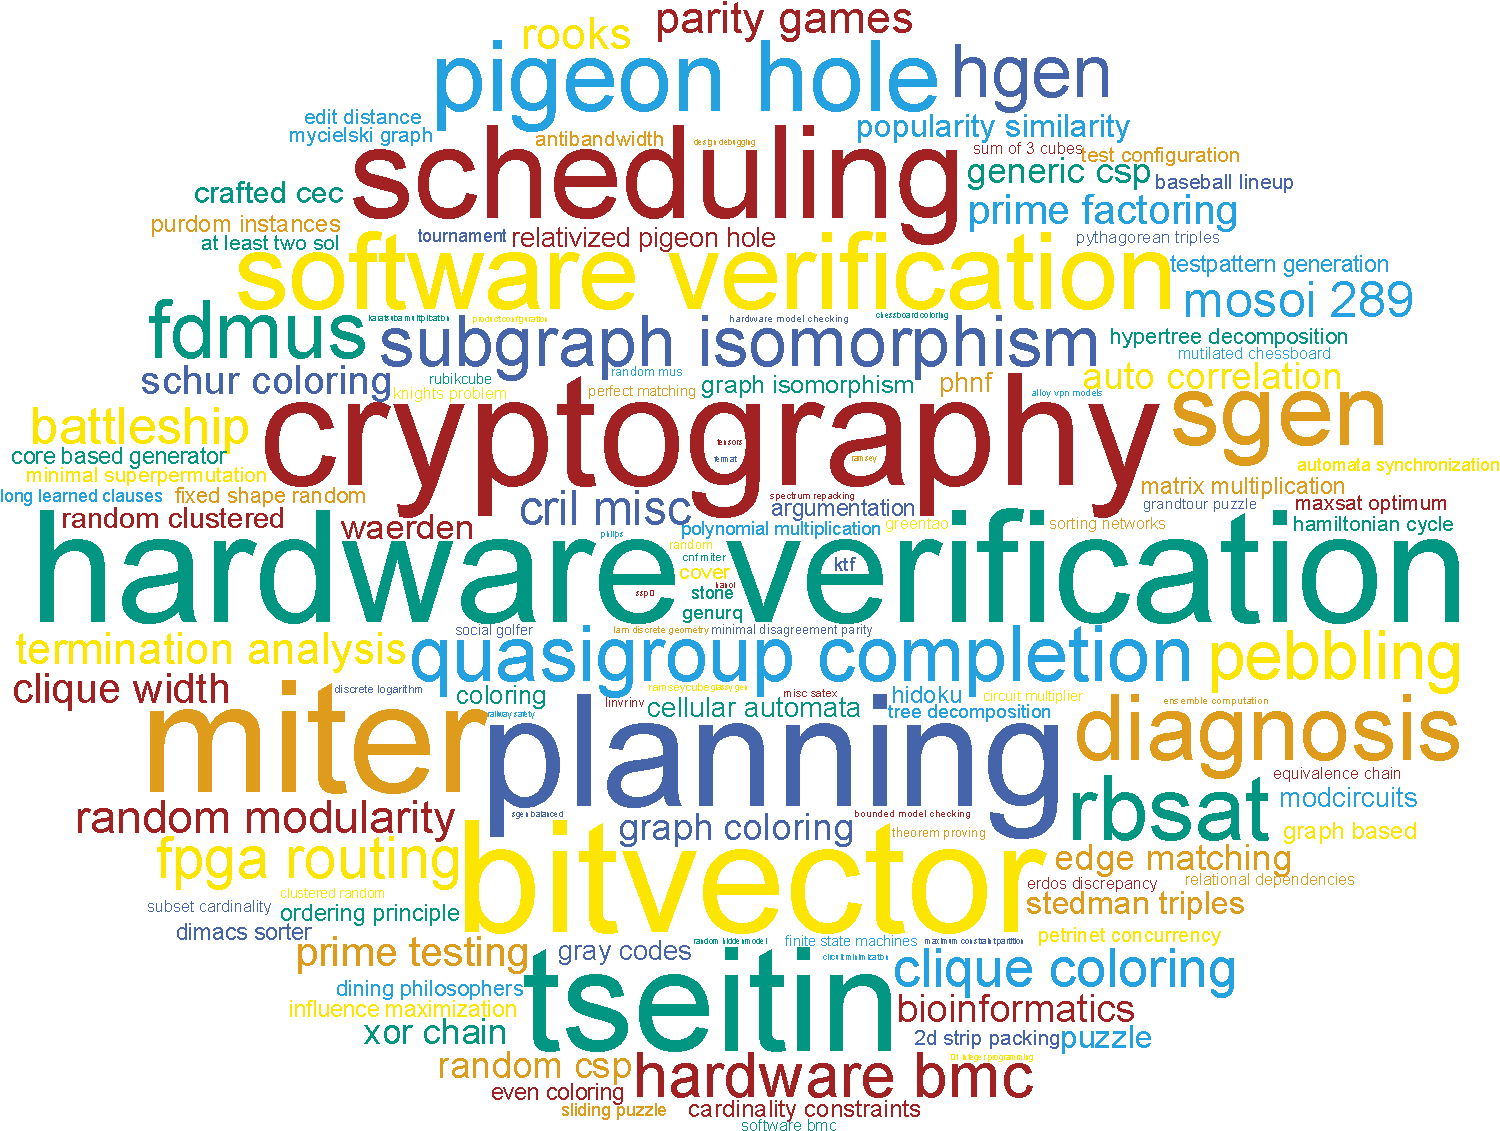
\includegraphics[height=13cm]{figures/l10/wordcloud3-crop.pdf}
	\end{minipage}%
	\begin{minipage}{0.27\textwidth}
		\centering
		{
			5355 problems,\\
			138 families + 72 unknown\\[3mm]
			Font size\ \,$\propto$\ \,\#\,problems\\[3mm]
			via \url{wordclouds.com},\\
			GBD (\url{benchmark-database.de})
		}
	\end{minipage}%
\end{frame}




\begin{frame}{Automated Planning: Introduction}
	\begin{blueblock}{Classical Automated Planning in a Nutshell}
		Given a \highl{set of world features}, an according \highl{initial world state}, and a set of \highl{conditional rules} to modify the world state (``\highl{actions}''),
		find a way to successively transform the initial world state until it satisfies some \highl{goal condition}.
	\end{blueblock}
	
	\vspace*{3mm}
	\textbf{Properties of (classical) automated planning:}
	\begin{itemize}
		\item Deterministic, full-knowledge, closed-world~\cite{reiter1981closed} (``\textit{everything not explicitly true is assumed false}'')
		\item Extremely generic ``\highl{state transition system}'' model
		\\-- essentially \highl{shortest path search} but on a prohibitively large graph that must be \highl{generated on the go}
		\item {\sffamily \textbf{PSPACE}}-complete~\cite{bylander1994computational} -- solutions may need to be \highlo{exponentially long}
		\item Applications of classical planning models mostly limited to \highlo{highly idealized/simplified settings}
		\\-- But: Ideal ``\highl{fruitfly problem}'' for considering interactions of applications with SAT solving
		\item Tons of extensions, enhancements, variants
	\end{itemize}
\end{frame}

\begin{frame}{Automated Planning: Definitions}
	\begin{blueblock}{Planning Problem (semi formal, simplified PDDL-style)}
		A \textbf{planning problem} is a tuple $P := (s_I, A, g)$, where $s_I$ and $g$ are \highl{sets of consistent propositional world state features} (each true or false) and $A$ is a \highl{set of actions}.
		Each action has the shape $a = (pre_a, eff_a)$, where $pre_a$ and $eff_a$ are also sets of consistent propositional world state features.
		The \textbf{objective} is to find a \highl{plan} $\Pi = \langle a_1, \ldots, a_n \rangle$ such that each $pre_{a_k}$ is satisfied by $s_k :=$ ($s_I$ updated by $eff_{a_1}, \ldots, eff_{a_{k-1}}$) and $g$ is satisfied by the final arising state $s_{n+1}$.
	\end{blueblock}
	
	\pause
	\vspace*{4mm}
	\begin{minipage}{0.6\textwidth}
		\begin{exampleblock}{Example: Sokoban~\cite{culberson1997sokoban}}
			\begin{itemize}
				\item \textbf{World state features:} Positions of walls, boxes, goals, player
				\item \textbf{Actions:} Walk and push. E.g., \texttt{push-right(x, y)}:
				\begin{itemize}
					\item Preconditions: \texttt{player-at(x,y)}, \texttt{box-at(x+1,y)}, $\neg$\texttt{wall-at(x+2,y)},\\ \phantom{Preconditions:} $\neg$\texttt{box-at(x+2,y)}
					\item Effects: \texttt{player-at(x+1,y), $\neg$\texttt{box-at(x+1,y)}, \texttt{box-at(x+2,y)}}
				\end{itemize}
				\item \textbf{Goal:} \texttt{box-at($x^*$,$y^*$)} for each marked location $(x^*, y^*)$
				\item \textbf{Plan:} Series of move/push actions leading to a goal state
			\end{itemize}
		\end{exampleblock}
	\end{minipage}\quad\quad
	\begin{minipage}{0.35\textwidth}
		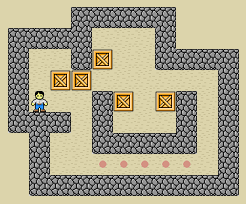
\includegraphics[width=0.8\textwidth]{figures/l10/sokoban.png}
	\end{minipage}%
\end{frame}

\begin{frame}{Automated Planning}
	\textbf{How do we solve planning problems?}
	\begin{itemize}
		\item Most common: \highl{Forward state space search}~\cite{helmert2006fast} -- explore state space while heuristically closing in on a goal state
		\item More exotic: Backward search, plan-space search (not discussed here)
		\item Old and robust (since 1992~\cite{kautz1992planning}): \highl{SAT-based planning}
	\end{itemize}
	\vspace*{5mm}
	\pause
	\textbf{(How) Can we encode planning problems into SAT?}
	\pause
	\begin{itemize}
		\item We cannot translate planning to a \highlo{single polynomially sized SAT encoding} (NP vs.~PSPACE?)\\
		-- \highlo{Unclear how many steps to encode!}
		\item We can translate planning to a compact SAT encoding \highl{for a fixed number of $K$ steps}
		\\$\Rightarrow$ \highl{Incrementally increase $K$} until plan is found!
		\item Main aspects of design space: Used SAT encoding, Scheduling strategies for values of $K$
	\end{itemize}
\end{frame}

\newcommand{\attime}[2]{{#1}^{(#2)}}

\begin{frame}{Automated Planning: A SAT Encoding~\cite{kautz1996pushing} (1/2)}
	\begin{enumerate}
		\item The \highl{initial state} has to hold at time $0$:\quad\unimp{(Assume $s_I$ explicitly defines \emph{all relevant/reachable propositions})}
		\[ \forall \ell \in s_I :\quad \attime{\ell}{0} \]
		\pause
		\item Apply \highl{at most one action} at each time:\quad\unimp{(Optionally also add ``\textit{At least one} action'')}
		\[ \forall t \in \{0,\ldots,K\}~~\forall a,a' \in A :\quad \neg \attime{a}{t} \vee \neg \attime{a'}{t} \]
		\pause
		\item Applying an action at time $t$ implies its \highl{preconditions at time $t$}:
		\[ \forall t \in \{0,\ldots,K\}~~\forall a \in A~~\forall \ell \in pre_a :\quad \attime{a}{t} \rightarrow \attime{\ell}{t} \]
		\pause
		\item Applying an action at time $t$ implies its \highl{effects at time $t+1$}:
		\[ \forall t \in \{0,\ldots,K\}~~\forall a \in A~~\forall \ell \in eff_a :\quad \attime{a}{t} \rightarrow \attime{\ell}{t+1} \]
		\pause
		\item Each \highl{goal} has to hold at time $K$:
		\[ \forall \ell \in g :\quad \attime{\ell}{K} \]
	\end{enumerate}
\end{frame}

\begin{frame}{Automated Planning: A SAT Encoding (2/2)}
	We are done, right?
	\pause
	
	$\Rightarrow$ Sokoban example: SAT Solver finds solution at $K=1$, where \highlo{boxes magically materialize at all goal spots}.

	What did we forget?
	\vspace*{4mm}
	\pause

	\begin{enumerate}
		\item[6.] \textbf{Frame axioms:} A state feature only changes if an action supports this change:
		\[ \forall t \in \{0,\ldots,K-1\}~~\forall \ell \in s_I \cup \bar{s_I} :\quad \attime{\bar{\ell}}{t} \wedge \attime{\ell}{t+1} \rightarrow \bigvee_{a \in A\ |\ \ell \in eff_a} \attime{a}{t} \]
	\end{enumerate}
	
	\pause
	\begin{blueblock}{Proposition}
		Using clause rules 1--6, encoding a planning problem $P$ to SAT for some fixed $K\geq 0$ yields a satisfiable CNF formula\\
		if and only if there exists a plan $\Pi$ for $P$ with at most $K$ steps.
		\\
		Such a $\Pi$ can be decoded from a model by reading the satisfying assignment to the variables $\attime{a}{t}$.
	\end{blueblock}
\end{frame}

\begin{frame}{SAT Planning}
	\begin{minipage}{0.6\textwidth}
		\textbf{Improvements to SAT-based planning}
		\begin{itemize}
			\item More efficient encodings, in particular for 2.~(``at most one action'')
			\item Relaxed semantics: Execute \highl{several actions at once} \unimp{(e.g.,}~\cite{balyo2013relaxing}\unimp{)}
			\vspace*{1.5mm}
			\item Exploit \highl{incremental SAT solving}!~\cite{gocht2017accelerating}
			\begin{itemize}
				\item Encode 1.~initially
				\item Encode 2.,3.,4.,6.~at every new increment
				\item Enforce 5.~(``goal reached'') as temporary \highl{assumptions} at each SAT call
			\end{itemize}
			\pause
			\item Find more effective \highl{sequences of values for $K$} to test\\
			(``\highl{makespan scheduling}'')~\cite{rintanen2004evaluation}
			\begin{itemize}
				\item Try to bypass \highlo{unsurmountable wall} of exceedingly difficult $K$ (esp.~UNSAT)
				\item Increase $K$ linearly, exponentially, \ldots
				\item Test several $K$ \highl{in parallel}
			\end{itemize}
		\end{itemize}
	\end{minipage}%
	\quad
	\begin{minipage}{0.35\textwidth}
		\vspace*{15mm}
		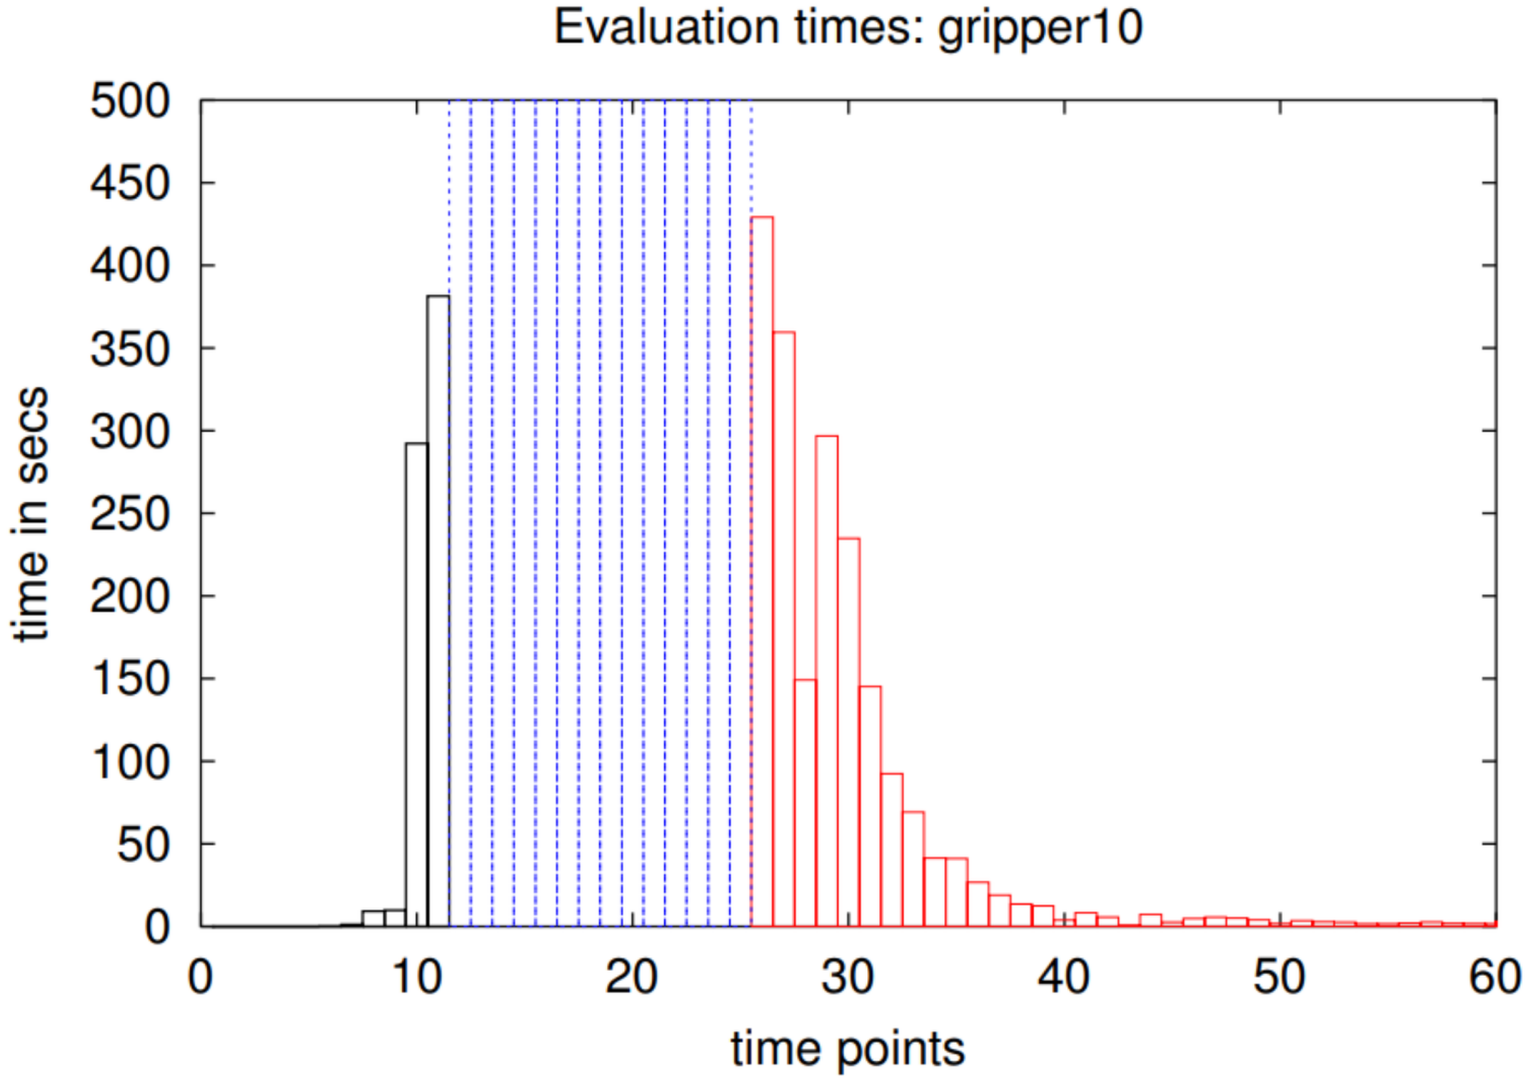
\includegraphics[width=\textwidth]{figures/l10/makespan-scheduling.png}
	\end{minipage}
\end{frame}

% https://link.springer.com/content/pdf/10.1023/A:1011276507260.pdf
\begin{frame}{From Planning to Verification?}
	\begin{minipage}[c][8cm][t]{0.65\textwidth}
		Let's use our SAT-based planning to \highl{check the correctness of a system}!
		\begin{itemize}
			\item World state features $\equiv$ State features of our system
			\item Actions $\equiv$ Valid \highl{transitions between states}
			\item Goals $\equiv$ \uncover<2->{\highl{incorrect state, violating some constraint}}
			\item<2-> Plan $\equiv$ \uncover<3->{\highlo{reachable incorrectness}}
			\item<3-> \highlo{Unsatisfiability}\only<4->{ \highlo{at $k$ steps}} $\equiv$ \only<3>{\highl{system is always correct?}}%
			\only<4->{\highl{system is correct \highlo{within $k$ steps}}}
		\end{itemize}
		\vspace*{3mm}
		\uncover<5->{
			\begin{block}{\textbf{Bounded Model Checking}}
				\begin{itemize}
					\item Encode and check \highl{transition system} for $k=1,2,\ldots$
					\item Satisfying assignment $\equiv$ \highlo{counter example}!
					\item Crucial tool for \highl{hardware and software verification}~\cite{vizel2015boolean}
				\end{itemize}
			\end{block}
		}
	\end{minipage}%
	\begin{minipage}[c][8cm][t]{0.35\textwidth}
		\centering
		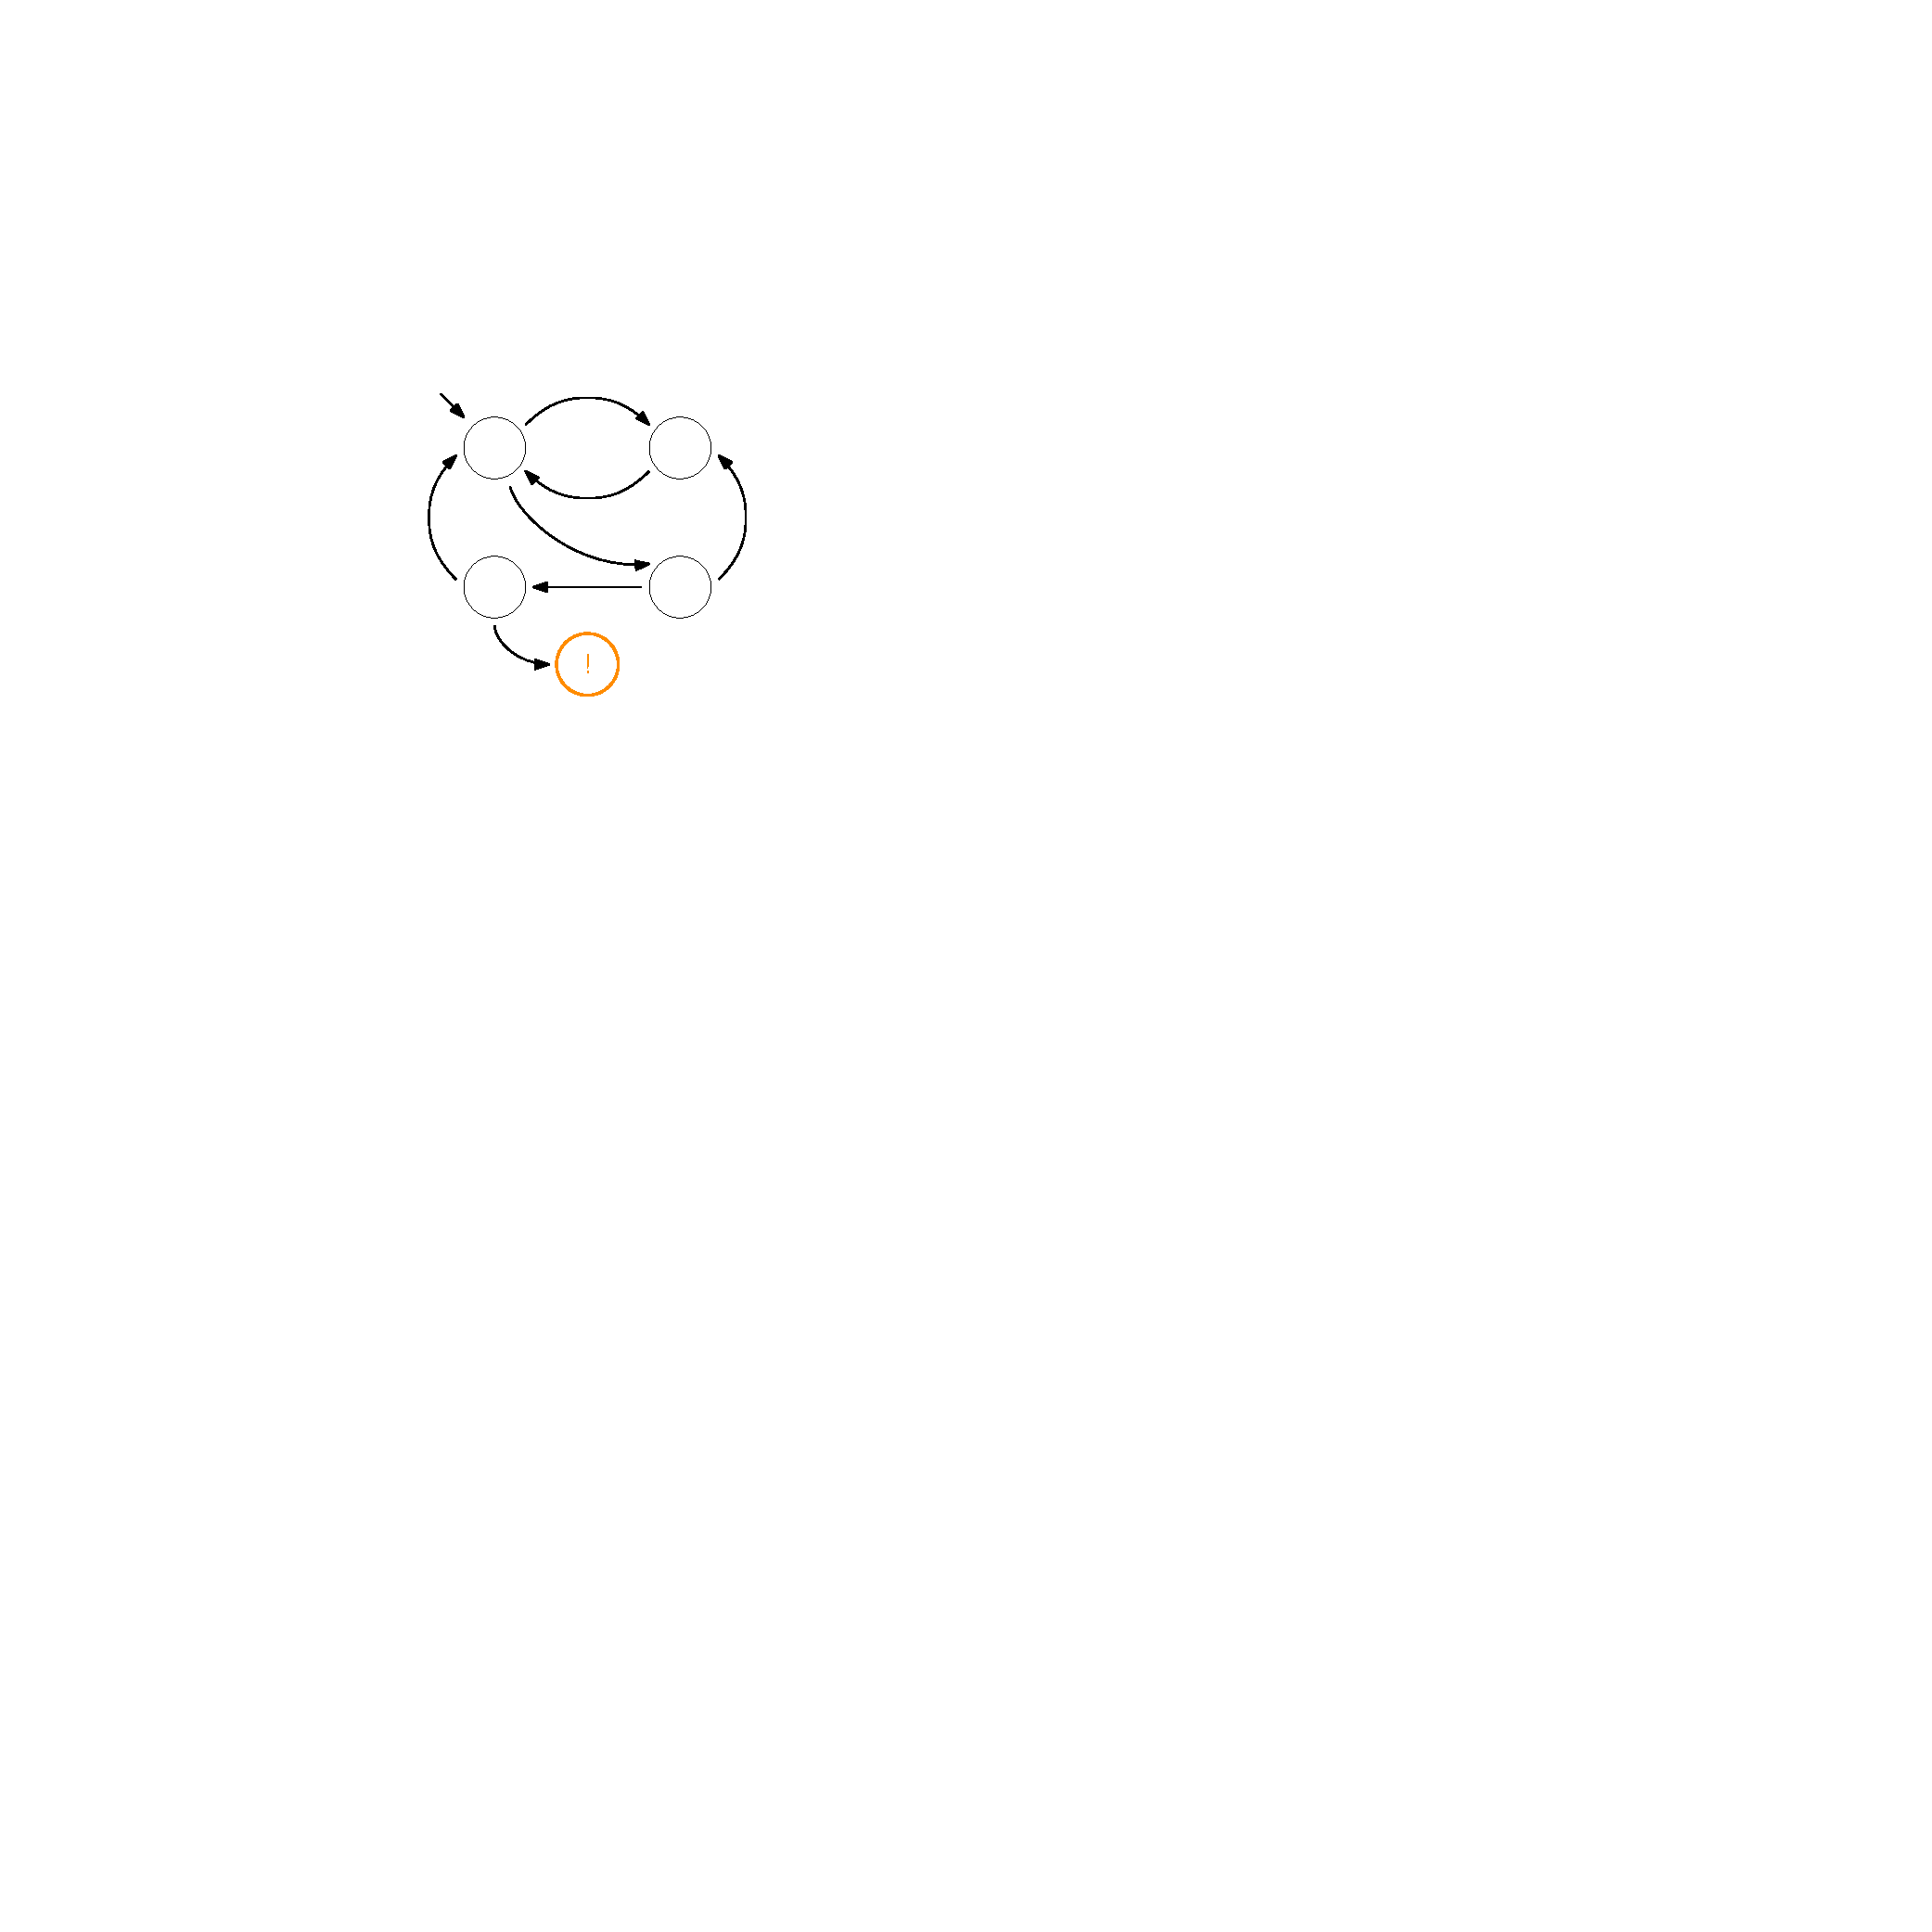
\includegraphics[width=0.9\textwidth]{figures/l10/transition-system-bmc.pdf}\\
		\textcolor{gray}{A snack machine or an electronic component or a C program or \ldots}
	\end{minipage}%
\end{frame}

\begin{frame}{Bounded Model Checking}
	\begin{minipage}[c][8cm][t]{0.6\textwidth}
		\begin{itemize}
			\item Invented by Clarke \& Biere in $\sim$2000~\cite{clarke2001bounded}, mostly replacing \highlo{BDD-based model checking}
			\item State transition system based on \highl{temporal logic}\\(LTL, CTL, \ldots);\ \ solving via \highl{SAT or SMT}
			\item Applications: Computer-aided design (CAD), software verification, invariant checking, bug detection, \ldots~\cite{vizel2015boolean}
			\item<2-> One of the \highl{most essential real-world applications} of SAT
			\begin{itemize}
				\item Pushed industrial interest in SAT solvers in 2000s
				\item Actively influenced solver design and algorithms
				\item Some of the \highl{largest, structurally most distinct} benchmarks
			\end{itemize}
			\item<3-> Examples for BMC @ KIT:
			\begin{itemize}
				\item \highl{Low-Level Bounded Model Checker} (LLBMC)~\cite{falke2013bounded}\\(C program verification)
				\item Verification of Java contracts~\cite{beckert2020modular} \unimp{(see right)}
				\item Cryptography~\cite{koch2021card}
			\end{itemize}
		\end{itemize}
	\end{minipage}%
	\begin{minipage}[c][8cm][t]{0.4\textwidth}
		\centering
		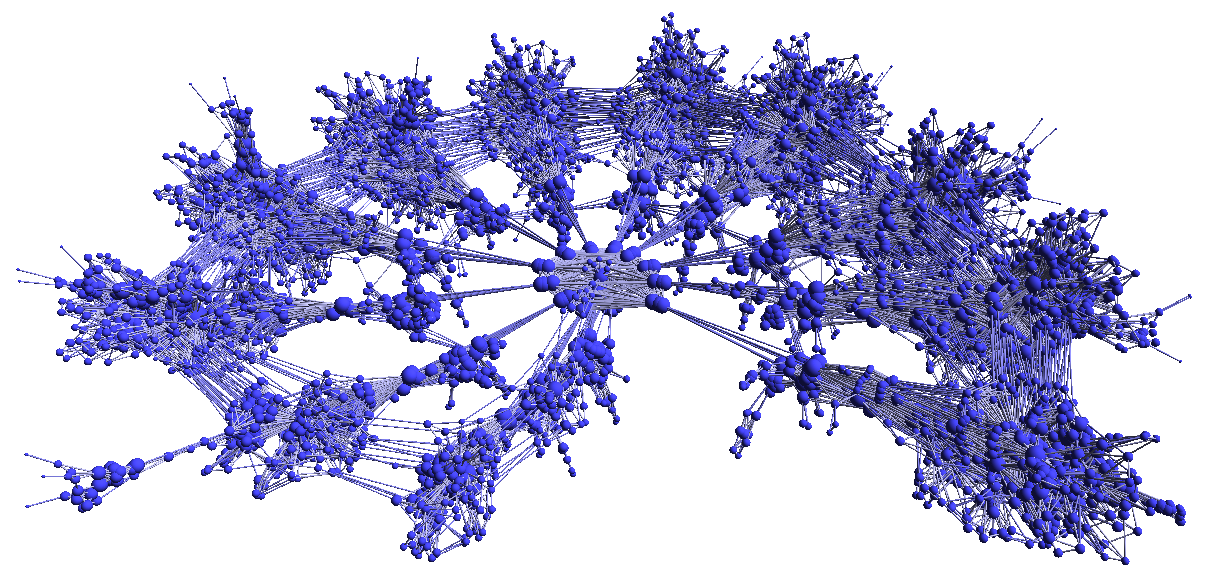
\includegraphics[width=0.9\textwidth]{figures/l10/bmc.png}
		%\\\textcolor{gray}{A Bounded Model Checking instance}
		\\[3mm]
		\uncover<3->{
			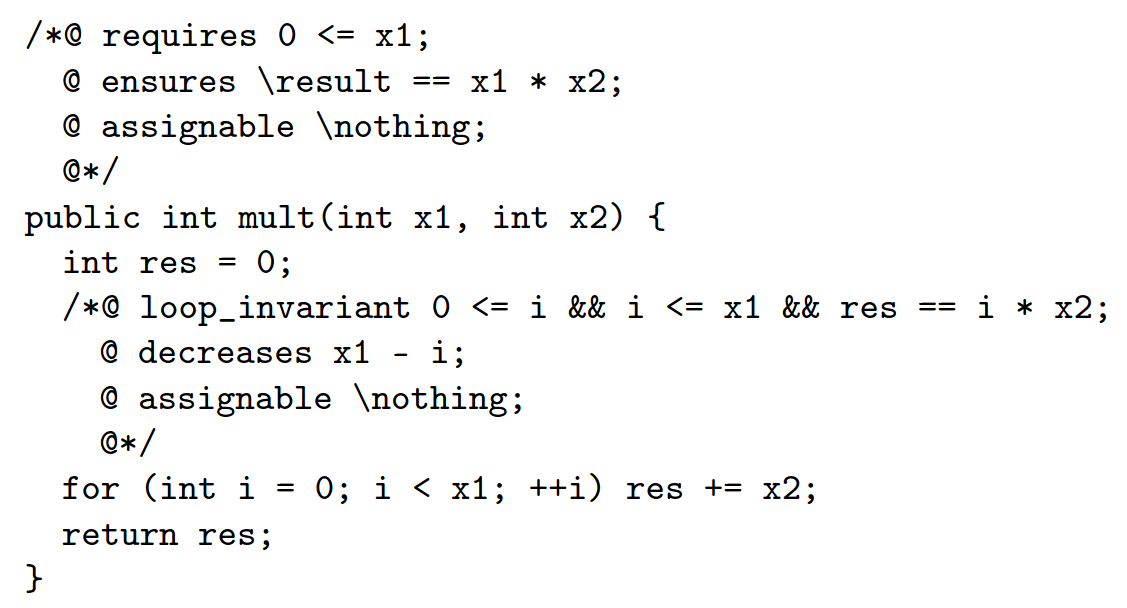
\includegraphics[width=\textwidth]{figures/l10/jml.png}
		}
	\end{minipage}%
\end{frame}






\begin{frame}{Recap}
	\begin{blueblock}{Applications I -- Planning \& Checking}
		\begin{itemize}\setlength{\itemsep}{1ex}
			\item Why consider applications?
			\item Automated planning: Foundations and SAT-based methods
			\item From planning to checking: Bounded Model Checking basics
		\end{itemize}
	\end{blueblock}
	
	\begin{block}{Next Up: Applications II -- Highlights}
		\begin{itemize}
			\item Electronic design
			\item Cryptanalysis
			\item Path finding and scheduling
			\item \ldots
		\end{itemize}
	\end{block}
\end{frame}


\begin{frame}[allowframebreaks]{References}
	\renewcommand*{\bibfont}{\footnotesize}
	\printbibliography[heading=subbibliography]
\end{frame}

\end{document}
